\chapter{Introduction}\label{intro}
%\Cref{fig:sample}
% What is the problem?
%\section{Background and Motivation}
The famous spectrum scarcity problem~\cite{SpectrumScarcity} along with significant spectrum under-utilization~\cite{valenta2010survey} (Figure~\ref{fig:SpectrumUnderutilization}~\cite{valenta2010survey}) in traditional spectrum management has lead towards the notion of dynamic spectrum access~\cite{akyildiz2006next} through cognitive radios. A \textit{cognitive radio} monitors its operational electromagnetic environment to dynamically adjust its operating parameters~\cite{Mitola}. Thus, a cognitive radio is capable of accessing temporal free spectrums. Cognitive Radio Networks (CRNs) exploit cognitive radios in their nodes for enabling access to temporal free spectrums. The typical architecture of CRNs comprises of two types of users as shown in Figure~\ref{fig:crn}. The first type of users refers to \textit{primary users} (PUs), who possess licenses to operate over different spectrum bands. The second type of users refers to \textit{secondary users} (SUs), who are unlicensed and employ cognitive radios to opportunistically access instantaneous spectrum holes.


\begin{figure}[!htbp]
    \begin{center}
        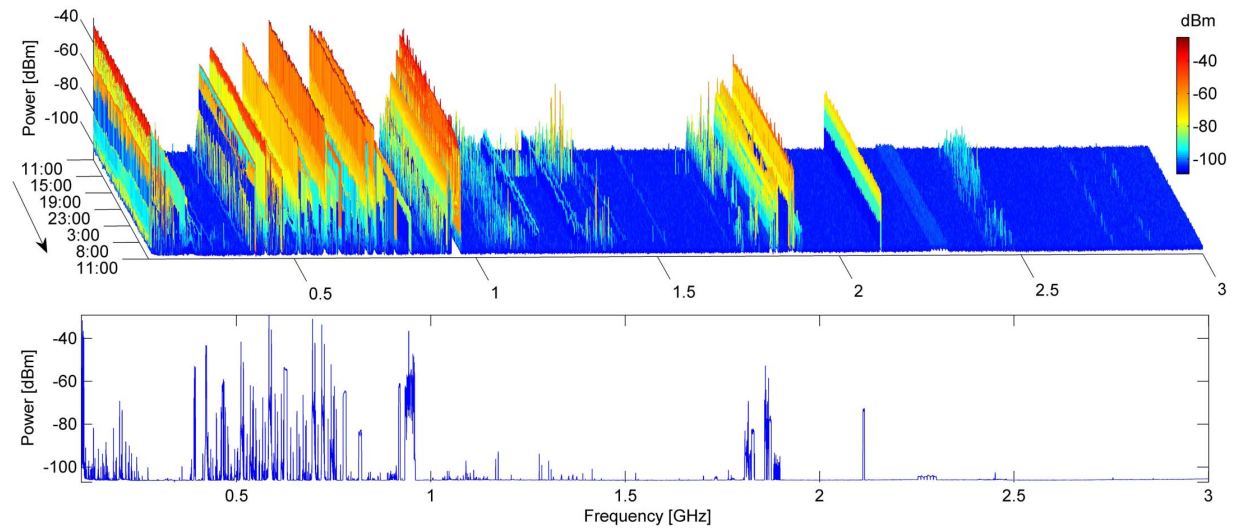
\includegraphics[width=0.8\textwidth]{myFigures/SpectrumUnderutilizationSir.PNG}
        \caption{Licensed frequency spectrums are mostly under-utilized}
        \label{fig:SpectrumUnderutilization}
    \end{center}
\end{figure}

\begin{figure}[!htbp]
    \begin{center}
        \noindent\begin{minipage}{\textwidth}
    \begin{minipage}[c][6cm][c]{\dimexpr0.33\textwidth-0.5\Colsep\relax}        
        \begin{subfigure}[c]{1.0\textwidth}
            
\begin{center}
    \begin{tikzpicture} [scale=0.8, transform shape]%show background rectangle,
        \tikzstyle{every node} = [draw, shape = rectangle, node distance=0mm, minimum width=5mm, minimum height=5.2mm]
        \node[draw=black, thick, label=below:Channel 2] (channel2) {
            \begin{tikzpicture}
                \node (puIdle) [fill=red!40, minimum width=30mm] {\small  Busy};%
            \end{tikzpicture}
        };
        \node[draw=black, thick, label=below:Channel 1] (channel1) [above=of channel2, yshift=7.5mm] {
            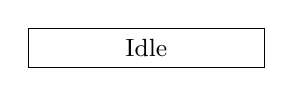
\begin{tikzpicture}
                \node (puBusy) [minimum width=30mm] {\small  Idle};
            \end{tikzpicture}
        };
        \node[draw=black, thick, label=below:Channel 3] (channel3) [below=of channel2, yshift=-7.5mm] {
            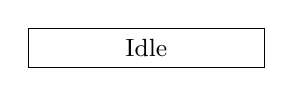
\begin{tikzpicture}
                \node (puBusy) [ minimum width=30mm] {\small  Idle};
            \end{tikzpicture}
        };
        \node[draw=black, thick, label=below:Channel 4] (channel4) [below=of channel3, yshift=-7.5mm] {
            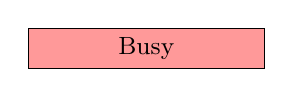
\begin{tikzpicture}
                \node (puBusy) [fill=red!40, minimum width=30mm] {\small  Busy};
            \end{tikzpicture}
        };

        \node[draw=white, thick] (pu1) [left=of channel1, xshift=-1mm] {
            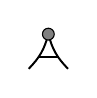
\begin{tikzpicture} [scale=0.5]
            \draw [line width=0.25mm, bend right = 15] (2, -0.44) to (2.5,0.44);
            \draw [line width=0.25mm, bend left = 15] (3, -0.44) to (2.5,0.44);
            \draw [line width=0.25mm] (2.25, -0.15) to (2.75,-0.15);
            %\draw [line width=0.25mm] (2.5, -0.44) to (2.5,0.44);
            \draw [fill=gray] (2.5,0.44) circle(1.5mm);

            \end{tikzpicture}
        };

        \node[draw=white, thick] (pu2) [left=of channel2, xshift=-1mm] {
            
\begin{tikzpicture} [scale=0.5]
            \draw [line width=0.25mm, bend right = 15, red] (2, -0.44) to (2.5,0.44);
            \draw [line width=0.25mm, bend left = 15, red] (3, -0.44) to (2.5,0.44);
            \draw [line width=0.25mm, red] (2.25, -0.15) to (2.75,-0.15);
            %\draw [line width=0.25mm] (2.5, -0.44) to (2.5,0.44);
            \draw [fill=red, red] (2.5,0.44) circle(1.5mm);

            \draw [line width=0.25mm, red] (2.5, 0.725) to (2.5,1.0);
            \draw [line width=0.25mm, red] (2.65, 0.65) to (2.825,0.85);
            \draw [line width=0.25mm, red] (2.725, 0.44) to (3,0.44);
            \draw [line width=0.25mm, red] (2.35, 0.65) to (2.175,0.85);
            \draw [line width=0.25mm, red] (2.275, 0.44) to (2,0.44);

            \end{tikzpicture}
        };

        \node[draw=white, thick] (pux1) [left=of pu2, xshift=-1mm] {
            
\begin{tikzpicture} [scale=0.5]
            \draw [line width=0.25mm, bend right = 15, red] (2, -0.44) to (2.5,0.44);
            \draw [line width=0.25mm, bend left = 15, red] (3, -0.44) to (2.5,0.44);
            \draw [line width=0.25mm, red] (2.15, -0.3) to (2.85,-0.3);
            \draw [line width=0.25mm, red] (2.25, -0.15) to (2.75,-0.15);
            \draw [line width=0.25mm, red] (2.35, 0) to (2.65,0);
            %\draw [line width=0.25mm] (2.5, -0.44) to (2.5,0.44);
            \draw [fill=red, red] (2.5,0.44) circle(1.5mm);

            \draw [line width=0.25mm, red] (2.5, 0.725) to (2.5,1.0);
            \draw [line width=0.25mm, red] (2.65, 0.65) to (2.825,0.85);
            \draw [line width=0.25mm, red] (2.725, 0.44) to (3,0.44);
            \draw [line width=0.25mm, red] (2.35, 0.65) to (2.175,0.85);
            \draw [line width=0.25mm, red] (2.275, 0.44) to (2,0.44);

            \end{tikzpicture}
        };

        \node[draw=white, thick] (pux2) [left=of pux1, xshift=-1mm] {
            
\begin{tikzpicture} [scale=0.5]
            \draw [line width=0.25mm, bend right = 15, red] (2, -0.44) to (2.5,0.44);
            \draw [line width=0.25mm, bend left = 15, red] (3, -0.44) to (2.5,0.44);
            \draw [line width=0.25mm, red] (2.15, -0.3) to (2.85,-0.3);
            \draw [line width=0.25mm, red] (2.25, -0.15) to (2.75,-0.15);
            \draw [line width=0.25mm, red] (2.35, 0) to (2.65,0);
            %\draw [line width=0.25mm] (2.5, -0.44) to (2.5,0.44);
            \draw [fill=red, red] (2.5,0.44) circle(1.5mm);

            \draw [line width=0.25mm, red] (2.5, 0.725) to (2.5,1.0);
            \draw [line width=0.25mm, red] (2.65, 0.65) to (2.825,0.85);
            \draw [line width=0.25mm, red] (2.725, 0.44) to (3,0.44);
            \draw [line width=0.25mm, red] (2.35, 0.65) to (2.175,0.85);
            \draw [line width=0.25mm, red] (2.275, 0.44) to (2,0.44);

            \end{tikzpicture}
        };

        \node[draw=white, thick] (pu3) [left=of channel3, xshift=-1mm] {
            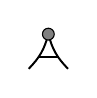
\begin{tikzpicture} [scale=0.5]
            \draw [line width=0.25mm, bend right = 15] (2, -0.44) to (2.5,0.44);
            \draw [line width=0.25mm, bend left = 15] (3, -0.44) to (2.5,0.44);
            \draw [line width=0.25mm] (2.25, -0.15) to (2.75,-0.15);
            %\draw [line width=0.25mm] (2.5, -0.44) to (2.5,0.44);
            \draw [fill=gray] (2.5,0.44) circle(1.5mm);

            \end{tikzpicture}
        };

        \node[draw=white, thick] (pu4) [left=of channel4, xshift=-1mm] {
            
\begin{tikzpicture} [scale=0.5]
            \draw [line width=0.25mm, bend right = 15, red] (2, -0.44) to (2.5,0.44);
            \draw [line width=0.25mm, bend left = 15, red] (3, -0.44) to (2.5,0.44);
            \draw [line width=0.25mm, red] (2.25, -0.15) to (2.75,-0.15);
            %\draw [line width=0.25mm] (2.5, -0.44) to (2.5,0.44);
            \draw [fill=red, red] (2.5,0.44) circle(1.5mm);

            \draw [line width=0.25mm, red] (2.5, 0.725) to (2.5,1.0);
            \draw [line width=0.25mm, red] (2.65, 0.65) to (2.825,0.85);
            \draw [line width=0.25mm, red] (2.725, 0.44) to (3,0.44);
            \draw [line width=0.25mm, red] (2.35, 0.65) to (2.175,0.85);
            \draw [line width=0.25mm, red] (2.275, 0.44) to (2,0.44);

            \end{tikzpicture}
        };
    \end{tikzpicture}
    \begin{tikzpicture}
    

        \iffalse
        \node[draw=white, thick, label=left:\tiny Primary User] (pu) [left=of pu3, xshift=-1cm] {
            \begin{tikzpicture} [scale=0.5]
            \draw [line width=0.25mm, bend right = 15] (2, -0.44) to (2.5,0.44);
            \draw [line width=0.25mm, bend left = 15] (3, -0.44) to (2.5,0.44);
            \draw [line width=0.25mm] (2.25, -0.15) to (2.75,-0.15);
            %\draw [line width=0.25mm] (2.5, -0.44) to (2.5,0.44);
            \draw [fill=gray] (2.5,0.44) circle(1.5mm);

            \end{tikzpicture}
        };

        \node[draw=white, thick] (su) [right=of su2, xshift=1cm, yshift=-1mm] {
            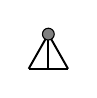
\begin{tikzpicture} [scale=0.5]
            \draw [line width=0.25mm] (2, -0.44) to (2.5,0.44);
            \draw [line width=0.25mm] (3, -0.44) to (2.5,0.44);
            \draw [line width=0.25mm] (2, -0.44) to (3,-0.44);
            \draw [line width=0.25mm] (2.5, -0.44) to (2.5,0.44);
            \draw [fill=gray] (2.5,0.44) circle(1.5mm);

            \end{tikzpicture}
        };
        \fi
    \end{tikzpicture}
\begin{center}
%\only<1>{In CRNs there are some Primary users and some Secondary users, some of the Primary users remain mostly Idle, where a Secondary user can operate.}
%\only<2>{If the Idleness of a Primary user change, the Secondary user's operation can get interrupted.}
%\only<3>{The secondary user need to switch to a new Idle channel.}
%\only<4>{Now. the question is what do we focus in such CRNs?}
\end{center}
\iffalse
\only<5>{
\begin{textblock*}{0.6\textwidth}(0.28\textwidth,0.4\textheight)
\textblockcolour{green!25!white}
\centering
\vspace{5mm}
  \textcolor{red}{Motivation}\\
  significant spectrum under-utilization in traditional spectrum management~\cite{akyildiz2006next}
\vspace{5mm}
\end{textblock*}
}
\fi
\end{center}

            \label{subfig:crnPU}
        \end{subfigure}
        %
\begin{center}
    \begin{tikzpicture} [scale=0.8, transform shape]%show background rectangle,
        \tikzstyle{every node} = [draw, shape = rectangle, node distance=0mm, minimum width=5mm, minimum height=5.2mm]
        \node[draw=black, thick, label=below:Channel 2] (channel2) {
            \begin{tikzpicture}
                \node (puIdle) [fill=red!40, minimum width=30mm] {\small  Busy};%
            \end{tikzpicture}
        };
        \node[draw=black, thick, label=below:Channel 1] (channel1) [above=of channel2, yshift=7.5mm] {
            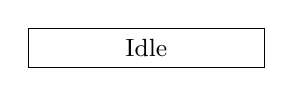
\begin{tikzpicture}
                \node (puBusy) [minimum width=30mm] {\small  Idle};
            \end{tikzpicture}
        };
        \node[draw=black, thick, label=below:Channel 3] (channel3) [below=of channel2, yshift=-7.5mm] {
            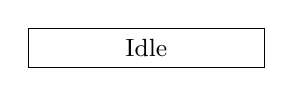
\begin{tikzpicture}
                \node (puBusy) [ minimum width=30mm] {\small  Idle};
            \end{tikzpicture}
        };
        \node[draw=black, thick, label=below:Channel 4] (channel4) [below=of channel3, yshift=-7.5mm] {
            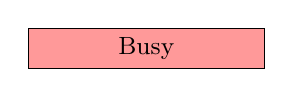
\begin{tikzpicture}
                \node (puBusy) [fill=red!40, minimum width=30mm] {\small  Busy};
            \end{tikzpicture}
        };

        \node[draw=white, thick] (pu1) [left=of channel1, xshift=-1mm] {
            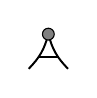
\begin{tikzpicture} [scale=0.5]
            \draw [line width=0.25mm, bend right = 15] (2, -0.44) to (2.5,0.44);
            \draw [line width=0.25mm, bend left = 15] (3, -0.44) to (2.5,0.44);
            \draw [line width=0.25mm] (2.25, -0.15) to (2.75,-0.15);
            %\draw [line width=0.25mm] (2.5, -0.44) to (2.5,0.44);
            \draw [fill=gray] (2.5,0.44) circle(1.5mm);

            \end{tikzpicture}
        };

        \node[draw=white, thick] (pu2) [left=of channel2, xshift=-1mm] {
            
\begin{tikzpicture} [scale=0.5]
            \draw [line width=0.25mm, bend right = 15, red] (2, -0.44) to (2.5,0.44);
            \draw [line width=0.25mm, bend left = 15, red] (3, -0.44) to (2.5,0.44);
            \draw [line width=0.25mm, red] (2.25, -0.15) to (2.75,-0.15);
            %\draw [line width=0.25mm] (2.5, -0.44) to (2.5,0.44);
            \draw [fill=red, red] (2.5,0.44) circle(1.5mm);

            \draw [line width=0.25mm, red] (2.5, 0.725) to (2.5,1.0);
            \draw [line width=0.25mm, red] (2.65, 0.65) to (2.825,0.85);
            \draw [line width=0.25mm, red] (2.725, 0.44) to (3,0.44);
            \draw [line width=0.25mm, red] (2.35, 0.65) to (2.175,0.85);
            \draw [line width=0.25mm, red] (2.275, 0.44) to (2,0.44);

            \end{tikzpicture}
        };

        \node[draw=white, thick] (pux1) [left=of pu2, xshift=-1mm] {
            
\begin{tikzpicture} [scale=0.5]
            \draw [line width=0.25mm, bend right = 15, red] (2, -0.44) to (2.5,0.44);
            \draw [line width=0.25mm, bend left = 15, red] (3, -0.44) to (2.5,0.44);
            \draw [line width=0.25mm, red] (2.15, -0.3) to (2.85,-0.3);
            \draw [line width=0.25mm, red] (2.25, -0.15) to (2.75,-0.15);
            \draw [line width=0.25mm, red] (2.35, 0) to (2.65,0);
            %\draw [line width=0.25mm] (2.5, -0.44) to (2.5,0.44);
            \draw [fill=red, red] (2.5,0.44) circle(1.5mm);

            \draw [line width=0.25mm, red] (2.5, 0.725) to (2.5,1.0);
            \draw [line width=0.25mm, red] (2.65, 0.65) to (2.825,0.85);
            \draw [line width=0.25mm, red] (2.725, 0.44) to (3,0.44);
            \draw [line width=0.25mm, red] (2.35, 0.65) to (2.175,0.85);
            \draw [line width=0.25mm, red] (2.275, 0.44) to (2,0.44);

            \end{tikzpicture}
        };

        \node[draw=white, thick] (pux2) [left=of pux1, xshift=-1mm] {
            
\begin{tikzpicture} [scale=0.5]
            \draw [line width=0.25mm, bend right = 15, red] (2, -0.44) to (2.5,0.44);
            \draw [line width=0.25mm, bend left = 15, red] (3, -0.44) to (2.5,0.44);
            \draw [line width=0.25mm, red] (2.15, -0.3) to (2.85,-0.3);
            \draw [line width=0.25mm, red] (2.25, -0.15) to (2.75,-0.15);
            \draw [line width=0.25mm, red] (2.35, 0) to (2.65,0);
            %\draw [line width=0.25mm] (2.5, -0.44) to (2.5,0.44);
            \draw [fill=red, red] (2.5,0.44) circle(1.5mm);

            \draw [line width=0.25mm, red] (2.5, 0.725) to (2.5,1.0);
            \draw [line width=0.25mm, red] (2.65, 0.65) to (2.825,0.85);
            \draw [line width=0.25mm, red] (2.725, 0.44) to (3,0.44);
            \draw [line width=0.25mm, red] (2.35, 0.65) to (2.175,0.85);
            \draw [line width=0.25mm, red] (2.275, 0.44) to (2,0.44);

            \end{tikzpicture}
        };

        \node[draw=white, thick] (pu3) [left=of channel3, xshift=-1mm] {
            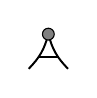
\begin{tikzpicture} [scale=0.5]
            \draw [line width=0.25mm, bend right = 15] (2, -0.44) to (2.5,0.44);
            \draw [line width=0.25mm, bend left = 15] (3, -0.44) to (2.5,0.44);
            \draw [line width=0.25mm] (2.25, -0.15) to (2.75,-0.15);
            %\draw [line width=0.25mm] (2.5, -0.44) to (2.5,0.44);
            \draw [fill=gray] (2.5,0.44) circle(1.5mm);

            \end{tikzpicture}
        };

        \node[draw=white, thick] (pu4) [left=of channel4, xshift=-1mm] {
            
\begin{tikzpicture} [scale=0.5]
            \draw [line width=0.25mm, bend right = 15, red] (2, -0.44) to (2.5,0.44);
            \draw [line width=0.25mm, bend left = 15, red] (3, -0.44) to (2.5,0.44);
            \draw [line width=0.25mm, red] (2.25, -0.15) to (2.75,-0.15);
            %\draw [line width=0.25mm] (2.5, -0.44) to (2.5,0.44);
            \draw [fill=red, red] (2.5,0.44) circle(1.5mm);

            \draw [line width=0.25mm, red] (2.5, 0.725) to (2.5,1.0);
            \draw [line width=0.25mm, red] (2.65, 0.65) to (2.825,0.85);
            \draw [line width=0.25mm, red] (2.725, 0.44) to (3,0.44);
            \draw [line width=0.25mm, red] (2.35, 0.65) to (2.175,0.85);
            \draw [line width=0.25mm, red] (2.275, 0.44) to (2,0.44);

            \end{tikzpicture}
        };
    \end{tikzpicture}
    \begin{tikzpicture}
    

        \iffalse
        \node[draw=white, thick, label=left:\tiny Primary User] (pu) [left=of pu3, xshift=-1cm] {
            \begin{tikzpicture} [scale=0.5]
            \draw [line width=0.25mm, bend right = 15] (2, -0.44) to (2.5,0.44);
            \draw [line width=0.25mm, bend left = 15] (3, -0.44) to (2.5,0.44);
            \draw [line width=0.25mm] (2.25, -0.15) to (2.75,-0.15);
            %\draw [line width=0.25mm] (2.5, -0.44) to (2.5,0.44);
            \draw [fill=gray] (2.5,0.44) circle(1.5mm);

            \end{tikzpicture}
        };

        \node[draw=white, thick] (su) [right=of su2, xshift=1cm, yshift=-1mm] {
            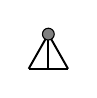
\begin{tikzpicture} [scale=0.5]
            \draw [line width=0.25mm] (2, -0.44) to (2.5,0.44);
            \draw [line width=0.25mm] (3, -0.44) to (2.5,0.44);
            \draw [line width=0.25mm] (2, -0.44) to (3,-0.44);
            \draw [line width=0.25mm] (2.5, -0.44) to (2.5,0.44);
            \draw [fill=gray] (2.5,0.44) circle(1.5mm);

            \end{tikzpicture}
        };
        \fi
    \end{tikzpicture}
\begin{center}
%\only<1>{In CRNs there are some Primary users and some Secondary users, some of the Primary users remain mostly Idle, where a Secondary user can operate.}
%\only<2>{If the Idleness of a Primary user change, the Secondary user's operation can get interrupted.}
%\only<3>{The secondary user need to switch to a new Idle channel.}
%\only<4>{Now. the question is what do we focus in such CRNs?}
\end{center}
\iffalse
\only<5>{
\begin{textblock*}{0.6\textwidth}(0.28\textwidth,0.4\textheight)
\textblockcolour{green!25!white}
\centering
\vspace{5mm}
  \textcolor{red}{Motivation}\\
  significant spectrum under-utilization in traditional spectrum management~\cite{akyildiz2006next}
\vspace{5mm}
\end{textblock*}
}
\fi
\end{center}

    \end{minipage}\hfill
    \begin{minipage}[c][6cm][c]{\dimexpr0.33\textwidth-0.5\Colsep\relax}      
        \begin{subfigure}[b]{1.0\textwidth}
            
\begin{center}
    \begin{tikzpicture} [scale=0.8, transform shape]%show background rectangle,
        \tikzstyle{every node} = [draw, shape = rectangle, node distance=0mm, minimum width=5mm, minimum height=5.2mm]
        \node[draw=black, thick, label=below:Channel 2] (channel2) {
            \begin{tikzpicture}
                \node (puIdle) [fill=red!40, minimum width=30mm] {\small  Busy};%
            \end{tikzpicture}
        };
        \node[draw=black, thick, label=below:Channel 1] (channel1) [above=of channel2, yshift=7.5mm] {
            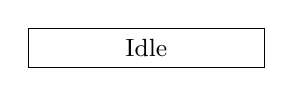
\begin{tikzpicture}
                \node (puBusy) [minimum width=30mm] {\small  Idle};
            \end{tikzpicture}
        };
        \node[draw=black, thick, label=below:Channel 3] (channel3) [below=of channel2, yshift=-7.5mm] {
            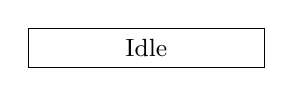
\begin{tikzpicture}
                \node (puBusy) [ minimum width=30mm] {\small  Idle};
            \end{tikzpicture}
        };
        \node[draw=black, thick, label=below:Channel 4] (channel4) [below=of channel3, yshift=-7.5mm] {
            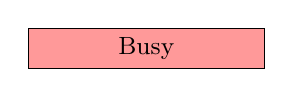
\begin{tikzpicture}
                \node (puBusy) [fill=red!40, minimum width=30mm] {\small  Busy};
            \end{tikzpicture}
        };

        \node[draw=white, thick] (pu1) [left=of channel1, xshift=-1mm] {
            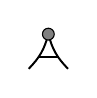
\begin{tikzpicture} [scale=0.5]
            \draw [line width=0.25mm, bend right = 15] (2, -0.44) to (2.5,0.44);
            \draw [line width=0.25mm, bend left = 15] (3, -0.44) to (2.5,0.44);
            \draw [line width=0.25mm] (2.25, -0.15) to (2.75,-0.15);
            %\draw [line width=0.25mm] (2.5, -0.44) to (2.5,0.44);
            \draw [fill=gray] (2.5,0.44) circle(1.5mm);

            \end{tikzpicture}
        };

        \node[draw=white, thick] (pu2) [left=of channel2, xshift=-1mm] {
            
\begin{tikzpicture} [scale=0.5]
            \draw [line width=0.25mm, bend right = 15, red] (2, -0.44) to (2.5,0.44);
            \draw [line width=0.25mm, bend left = 15, red] (3, -0.44) to (2.5,0.44);
            \draw [line width=0.25mm, red] (2.25, -0.15) to (2.75,-0.15);
            %\draw [line width=0.25mm] (2.5, -0.44) to (2.5,0.44);
            \draw [fill=red, red] (2.5,0.44) circle(1.5mm);

            \draw [line width=0.25mm, red] (2.5, 0.725) to (2.5,1.0);
            \draw [line width=0.25mm, red] (2.65, 0.65) to (2.825,0.85);
            \draw [line width=0.25mm, red] (2.725, 0.44) to (3,0.44);
            \draw [line width=0.25mm, red] (2.35, 0.65) to (2.175,0.85);
            \draw [line width=0.25mm, red] (2.275, 0.44) to (2,0.44);

            \end{tikzpicture}
        };

        \node[draw=white, thick] (pux1) [left=of pu2, xshift=-1mm] {
            
\begin{tikzpicture} [scale=0.5]
            \draw [line width=0.25mm, bend right = 15, red] (2, -0.44) to (2.5,0.44);
            \draw [line width=0.25mm, bend left = 15, red] (3, -0.44) to (2.5,0.44);
            \draw [line width=0.25mm, red] (2.15, -0.3) to (2.85,-0.3);
            \draw [line width=0.25mm, red] (2.25, -0.15) to (2.75,-0.15);
            \draw [line width=0.25mm, red] (2.35, 0) to (2.65,0);
            %\draw [line width=0.25mm] (2.5, -0.44) to (2.5,0.44);
            \draw [fill=red, red] (2.5,0.44) circle(1.5mm);

            \draw [line width=0.25mm, red] (2.5, 0.725) to (2.5,1.0);
            \draw [line width=0.25mm, red] (2.65, 0.65) to (2.825,0.85);
            \draw [line width=0.25mm, red] (2.725, 0.44) to (3,0.44);
            \draw [line width=0.25mm, red] (2.35, 0.65) to (2.175,0.85);
            \draw [line width=0.25mm, red] (2.275, 0.44) to (2,0.44);

            \end{tikzpicture}
        };

        \node[draw=white, thick] (pux2) [left=of pux1, xshift=-1mm] {
            
\begin{tikzpicture} [scale=0.5]
            \draw [line width=0.25mm, bend right = 15, red] (2, -0.44) to (2.5,0.44);
            \draw [line width=0.25mm, bend left = 15, red] (3, -0.44) to (2.5,0.44);
            \draw [line width=0.25mm, red] (2.15, -0.3) to (2.85,-0.3);
            \draw [line width=0.25mm, red] (2.25, -0.15) to (2.75,-0.15);
            \draw [line width=0.25mm, red] (2.35, 0) to (2.65,0);
            %\draw [line width=0.25mm] (2.5, -0.44) to (2.5,0.44);
            \draw [fill=red, red] (2.5,0.44) circle(1.5mm);

            \draw [line width=0.25mm, red] (2.5, 0.725) to (2.5,1.0);
            \draw [line width=0.25mm, red] (2.65, 0.65) to (2.825,0.85);
            \draw [line width=0.25mm, red] (2.725, 0.44) to (3,0.44);
            \draw [line width=0.25mm, red] (2.35, 0.65) to (2.175,0.85);
            \draw [line width=0.25mm, red] (2.275, 0.44) to (2,0.44);

            \end{tikzpicture}
        };
        
        \draw [line width=0.5mm, dashed, ->] (pux1) to (channel1);
        \draw [line width=0.5mm, dashed, ->] (pux2) to (channel3);

        \node[draw=white, thick] (pu3) [left=of channel3, xshift=-1mm] {
            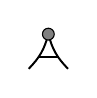
\begin{tikzpicture} [scale=0.5]
            \draw [line width=0.25mm, bend right = 15] (2, -0.44) to (2.5,0.44);
            \draw [line width=0.25mm, bend left = 15] (3, -0.44) to (2.5,0.44);
            \draw [line width=0.25mm] (2.25, -0.15) to (2.75,-0.15);
            %\draw [line width=0.25mm] (2.5, -0.44) to (2.5,0.44);
            \draw [fill=gray] (2.5,0.44) circle(1.5mm);

            \end{tikzpicture}
        };

        \node[draw=white, thick] (pu4) [left=of channel4, xshift=-1mm] {
            
\begin{tikzpicture} [scale=0.5]
            \draw [line width=0.25mm, bend right = 15, red] (2, -0.44) to (2.5,0.44);
            \draw [line width=0.25mm, bend left = 15, red] (3, -0.44) to (2.5,0.44);
            \draw [line width=0.25mm, red] (2.25, -0.15) to (2.75,-0.15);
            %\draw [line width=0.25mm] (2.5, -0.44) to (2.5,0.44);
            \draw [fill=red, red] (2.5,0.44) circle(1.5mm);

            \draw [line width=0.25mm, red] (2.5, 0.725) to (2.5,1.0);
            \draw [line width=0.25mm, red] (2.65, 0.65) to (2.825,0.85);
            \draw [line width=0.25mm, red] (2.725, 0.44) to (3,0.44);
            \draw [line width=0.25mm, red] (2.35, 0.65) to (2.175,0.85);
            \draw [line width=0.25mm, red] (2.275, 0.44) to (2,0.44);

            \end{tikzpicture}
        };
        
        
    \end{tikzpicture}
    \begin{tikzpicture}
    

        \iffalse
        \node[draw=white, thick, label=left:\tiny Primary User] (pu) [left=of pu3, xshift=-1cm] {
            \begin{tikzpicture} [scale=0.5]
            \draw [line width=0.25mm, bend right = 15] (2, -0.44) to (2.5,0.44);
            \draw [line width=0.25mm, bend left = 15] (3, -0.44) to (2.5,0.44);
            \draw [line width=0.25mm] (2.25, -0.15) to (2.75,-0.15);
            %\draw [line width=0.25mm] (2.5, -0.44) to (2.5,0.44);
            \draw [fill=gray] (2.5,0.44) circle(1.5mm);

            \end{tikzpicture}
        };

        \node[draw=white, thick] (su) [right=of su2, xshift=1cm, yshift=-1mm] {
            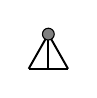
\begin{tikzpicture} [scale=0.5]
            \draw [line width=0.25mm] (2, -0.44) to (2.5,0.44);
            \draw [line width=0.25mm] (3, -0.44) to (2.5,0.44);
            \draw [line width=0.25mm] (2, -0.44) to (3,-0.44);
            \draw [line width=0.25mm] (2.5, -0.44) to (2.5,0.44);
            \draw [fill=gray] (2.5,0.44) circle(1.5mm);

            \end{tikzpicture}
        };
        \fi
    \end{tikzpicture}
\begin{center}
%\only<1>{In CRNs there are some Primary users and some Secondary users, some of the Primary users remain mostly Idle, where a Secondary user can operate.}
%\only<2>{If the Idleness of a Primary user change, the Secondary user's operation can get interrupted.}
%\only<3>{The secondary user need to switch to a new Idle channel.}
%\only<4>{Now. the question is what do we focus in such CRNs?}
\end{center}
\iffalse
\only<5>{
\begin{textblock*}{0.6\textwidth}(0.28\textwidth,0.4\textheight)
\textblockcolour{green!25!white}
\centering
\vspace{5mm}
  \textcolor{red}{Motivation}\\
  significant spectrum under-utilization in traditional spectrum management~\cite{akyildiz2006next}
\vspace{5mm}
\end{textblock*}
}
\fi
\end{center}

            \label{subfig:crnPUIntermediate}
        \end{subfigure}
    \end{minipage}\hfill
    \begin{minipage}[c][6cm][c]{\dimexpr0.33\textwidth-0.5\Colsep\relax}      
        \begin{subfigure}[b]{1.0\textwidth}
            
\begin{center}
    \begin{tikzpicture} [scale=0.8, transform shape]%show background rectangle,
        \tikzstyle{every node} = [draw, shape = rectangle, node distance=0mm, minimum width=5mm, minimum height=5.2mm]
        \node[draw=black, thick, label=below:Channel 2] (channel2) {
            \begin{tikzpicture}
                \node (puIdle) [fill=red!40, minimum width=30mm] {\small  Busy};%
            \end{tikzpicture}
        };
        \node[draw=black, thick, label=below:Channel 1] (channel1) [above=of channel2, yshift=7.5mm] {
            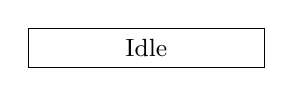
\begin{tikzpicture}
                \node (puBusy) [minimum width=30mm] {\small  Idle};
            \end{tikzpicture}
        };
        \node[draw=black, thick, label=below:Channel 3] (channel3) [below=of channel2, yshift=-7.5mm] {
            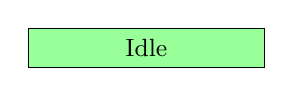
\begin{tikzpicture}
                \node (puBusy) [fill=green!40, minimum width=30mm] {\small  Idle};
            \end{tikzpicture}
        };
        \node[draw=black, thick, label=below:Channel 4] (channel4) [below=of channel3, yshift=-7.5mm] {
            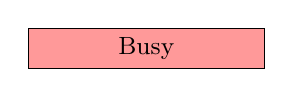
\begin{tikzpicture}
                \node (puBusy) [fill=red!40, minimum width=30mm] {\small  Busy};
            \end{tikzpicture}
        };
        
        \node[draw=white, thick] (sux1) [right=of channel1, xshift=1mm] {
            
\begin{tikzpicture} [scale=0.5]
            \draw [line width=0.25mm, green!50!black] (2, -0.44) to (2.5,0.44);
            \draw [line width=0.25mm, green!50!black] (3, -0.44) to (2.5,0.44);
            \draw [line width=0.25mm, green!50!black] (2, -0.44) to (3,-0.44);
            \draw [line width=0.25mm, green!50!black] (2.5, -0.44) to (2.5,0.44);
            \draw [fill=green!50!black, green!50!black] (2.5,0.44) circle(1.5mm);

            \draw [line width=0.25mm, green!50!black] (2.5, 0.725) to (2.5,1.0);
            \draw [line width=0.25mm, green!50!black] (2.65, 0.65) to (2.825,0.85);
            \draw [line width=0.25mm, green!50!black] (2.725, 0.44) to (3,0.44);
            \draw [line width=0.25mm, green!50!black] (2.35, 0.65) to (2.175,0.85);
            \draw [line width=0.25mm, green!50!black] (2.275, 0.44) to (2,0.44);

            \end{tikzpicture}
        };

        \node[draw=white, thick] (su2) [right=of channel3, xshift=1mm] {
            
\begin{tikzpicture} [scale=0.5]
            \draw [line width=0.25mm, green!50!black] (2, -0.44) to (2.5,0.44);
            \draw [line width=0.25mm, green!50!black] (3, -0.44) to (2.5,0.44);
            \draw [line width=0.25mm, green!50!black] (2, -0.44) to (3,-0.44);
            \draw [line width=0.25mm, green!50!black] (2.5, -0.44) to (2.5,0.44);
            \draw [fill=green!50!black, green!50!black] (2.5,0.44) circle(1.5mm);

            \draw [line width=0.25mm, green!50!black] (2.5, 0.725) to (2.5,1.0);
            \draw [line width=0.25mm, green!50!black] (2.65, 0.65) to (2.825,0.85);
            \draw [line width=0.25mm, green!50!black] (2.725, 0.44) to (3,0.44);
            \draw [line width=0.25mm, green!50!black] (2.35, 0.65) to (2.175,0.85);
            \draw [line width=0.25mm, green!50!black] (2.275, 0.44) to (2,0.44);

            \end{tikzpicture}
        };

        \node[draw=white, thick] (pu1) [left=of channel1, xshift=-1mm] {
            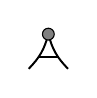
\begin{tikzpicture} [scale=0.5]
            \draw [line width=0.25mm, bend right = 15] (2, -0.44) to (2.5,0.44);
            \draw [line width=0.25mm, bend left = 15] (3, -0.44) to (2.5,0.44);
            \draw [line width=0.25mm] (2.25, -0.15) to (2.75,-0.15);
            %\draw [line width=0.25mm] (2.5, -0.44) to (2.5,0.44);
            \draw [fill=gray] (2.5,0.44) circle(1.5mm);

            \end{tikzpicture}
        };

        \node[draw=white, thick] (pu2) [left=of channel2, xshift=-1mm] {
            
\begin{tikzpicture} [scale=0.5]
            \draw [line width=0.25mm, bend right = 15, red] (2, -0.44) to (2.5,0.44);
            \draw [line width=0.25mm, bend left = 15, red] (3, -0.44) to (2.5,0.44);
            \draw [line width=0.25mm, red] (2.25, -0.15) to (2.75,-0.15);
            %\draw [line width=0.25mm] (2.5, -0.44) to (2.5,0.44);
            \draw [fill=red, red] (2.5,0.44) circle(1.5mm);

            \draw [line width=0.25mm, red] (2.5, 0.725) to (2.5,1.0);
            \draw [line width=0.25mm, red] (2.65, 0.65) to (2.825,0.85);
            \draw [line width=0.25mm, red] (2.725, 0.44) to (3,0.44);
            \draw [line width=0.25mm, red] (2.35, 0.65) to (2.175,0.85);
            \draw [line width=0.25mm, red] (2.275, 0.44) to (2,0.44);

            \end{tikzpicture}
        };

        \node[draw=white, thick] (pu3) [left=of channel3, xshift=-1mm] {
            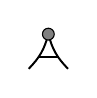
\begin{tikzpicture} [scale=0.5]
            \draw [line width=0.25mm, bend right = 15] (2, -0.44) to (2.5,0.44);
            \draw [line width=0.25mm, bend left = 15] (3, -0.44) to (2.5,0.44);
            \draw [line width=0.25mm] (2.25, -0.15) to (2.75,-0.15);
            %\draw [line width=0.25mm] (2.5, -0.44) to (2.5,0.44);
            \draw [fill=gray] (2.5,0.44) circle(1.5mm);

            \end{tikzpicture}
        };

        \node[draw=white, thick, label=below:PUs] (pu4) [left=of channel4, xshift=-1mm] {
            
\begin{tikzpicture} [scale=0.5]
            \draw [line width=0.25mm, bend right = 15, red] (2, -0.44) to (2.5,0.44);
            \draw [line width=0.25mm, bend left = 15, red] (3, -0.44) to (2.5,0.44);
            \draw [line width=0.25mm, red] (2.25, -0.15) to (2.75,-0.15);
            %\draw [line width=0.25mm] (2.5, -0.44) to (2.5,0.44);
            \draw [fill=red, red] (2.5,0.44) circle(1.5mm);

            \draw [line width=0.25mm, red] (2.5, 0.725) to (2.5,1.0);
            \draw [line width=0.25mm, red] (2.65, 0.65) to (2.825,0.85);
            \draw [line width=0.25mm, red] (2.725, 0.44) to (3,0.44);
            \draw [line width=0.25mm, red] (2.35, 0.65) to (2.175,0.85);
            \draw [line width=0.25mm, red] (2.275, 0.44) to (2,0.44);

            \end{tikzpicture}
        };

        \node[draw=white, thick, label=below:SUs] (suLabel) [right=of channel4, xshift=1mm] {
            \begin{tikzpicture} [scale=0.5]
            \draw [line width=0.25mm, white] (2, -0.44) to (2.5,0.44);
            \draw [line width=0.25mm, white] (3, -0.44) to (2.5,0.44);
            \draw [line width=0.25mm, white] (2, -0.44) to (3,-0.44);
            \draw [line width=0.25mm, white] (2.5, -0.44) to (2.5,0.44);
            \draw [fill=green!50!black, white] (2.5,0.44) circle(1.5mm);

            \draw [line width=0.25mm, white] (2.5, 0.725) to (2.5,1.0);
            \draw [line width=0.25mm, white] (2.65, 0.65) to (2.825,0.85);
            \draw [line width=0.25mm, white] (2.725, 0.44) to (3,0.44);
            \draw [line width=0.25mm, white] (2.35, 0.65) to (2.175,0.85);
            \draw [line width=0.25mm, white] (2.275, 0.44) to (2,0.44);

            \end{tikzpicture}
        };
    \end{tikzpicture}
    \begin{tikzpicture}
    

        \iffalse
        \node[draw=white, thick, label=left:\tiny Primary User] (pu) [left=of pu3, xshift=-1cm] {
            \begin{tikzpicture} [scale=0.5]
            \draw [line width=0.25mm, bend right = 15] (2, -0.44) to (2.5,0.44);
            \draw [line width=0.25mm, bend left = 15] (3, -0.44) to (2.5,0.44);
            \draw [line width=0.25mm] (2.25, -0.15) to (2.75,-0.15);
            %\draw [line width=0.25mm] (2.5, -0.44) to (2.5,0.44);
            \draw [fill=gray] (2.5,0.44) circle(1.5mm);

            \end{tikzpicture}
        };

        \node[draw=white, thick] (su) [right=of su2, xshift=1cm, yshift=-1mm] {
            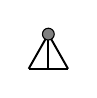
\begin{tikzpicture} [scale=0.5]
            \draw [line width=0.25mm] (2, -0.44) to (2.5,0.44);
            \draw [line width=0.25mm] (3, -0.44) to (2.5,0.44);
            \draw [line width=0.25mm] (2, -0.44) to (3,-0.44);
            \draw [line width=0.25mm] (2.5, -0.44) to (2.5,0.44);
            \draw [fill=gray] (2.5,0.44) circle(1.5mm);

            \end{tikzpicture}
        };
        \fi
    \end{tikzpicture}
\begin{center}
%\only<1>{In CRNs there are some Primary users and some Secondary users, some of the Primary users remain mostly Idle, where a Secondary user can operate.}
%\only<2>{If the Idleness of a Primary user change, the Secondary user's operation can get interrupted.}
%\only<3>{The secondary user need to switch to a new Idle channel.}
%\only<4>{Now. the question is what do we focus in such CRNs?}
\end{center}
\iffalse
\only<5>{
\begin{textblock*}{0.6\textwidth}(0.28\textwidth,0.4\textheight)
\textblockcolour{green!25!white}
\centering
\vspace{5mm}
  \textcolor{red}{Motivation}\\
  significant spectrum under-utilization in traditional spectrum management~\cite{akyildiz2006next}
\vspace{5mm}
\end{textblock*}
}
\fi
\end{center}

            \label{subfig:crnSU}
        \end{subfigure}
    \end{minipage}%
\end{minipage}

        \caption{Dynamic spectrum access through cognitive radio networks}
        \label{fig:crn}
    \end{center}
\end{figure}

% Why is it interesting and important?
%The importance of our study lies on the fact that almost all the modern mobile devices contain multiple radios.

On the other hand, classical wireless networks frequently adopt the notion of deploying users with multiple radios~\cite{bahl2004reconsidering, adya2004multi}. Such deployment of multiple radios improves capacity of the networks \cite{draves2004routing, bahl2004reconsidering}, enhances loss resilience \cite{miu2005improving}, and enables heterogeneous wireless access for smart devices \cite{song2012performance} (Figure~\ref{fig:advMRN}). As such deployment of multiple radios in wireless nodes is known to improve the performance of a user and  deployment of cognitive radios also aims to improve the performance of secondary users through spectrum utilization, it is intuitive that simultaneous utilization of both these techniques, i.e., Multi-Radio Cognitive Radio Networks (MRCRNs), will result in significantly improved network performance. Therefore, the notion of exploiting multiple radios in CRNs to supplement the dynamic spectrum access has been proposed in the contemporary literature~\cite{li2014deterministic, zhong2014capacity, khan2015towards}. Existing studies in this regard present that such multi-radio deployment in CRNs improves delay up to a certain point, however, throughput always degrades with an increase in the number of radios per secondary user~\cite{khan2015towards}. Therefore, examining how to improve network throughput while equipping secondary users with multiple radios still remains an open research problem in the literature.

\begin{figure*}[!htbp]
    \centering
    \begin{subfigure}[t]{0.3\textwidth}
            \begin{center}
        \begin{tikzpicture} [scale=1.0, transform shape]%show background rectangle,
        \tikzstyle{every node} = [draw, shape = rectangle, node distance=0mm, minimum width=4mm, minimum height=5mm]
        \node[draw=black, thick, label=below:\tiny Channel 1, minimum width=25mm] (channel1) {
        };
        \node[draw=black, thick, label=below:\tiny Channel 2, minimum width=25mm, fill=green!50] (channel2) [below=of channel1, yshift=-5mm] {
        };
        \node[draw=black, thick, label=below:\tiny Channel 3, minimum width=25mm, fill=green!50] (channel3) [below=of channel2, yshift=-5mm] {
        };
        \node[draw=black, thick, label=below:\tiny Channel 4, minimum width=25mm] (channel4) [below=of channel3, yshift=-5mm] {
        };
        \node[draw=white, thick] (su1) [left=of channel2, xshift=-1.5mm, yshift=0.5mm] {
            \begin{tikzpicture} [scale=0.5]
            \draw [line width=0.25mm, green!50!black] (2, -0.44) to (2.5,0.44);
            \draw [line width=0.25mm, green!50!black] (3, -0.44) to (2.5,0.44);
            \draw [line width=0.25mm, green!50!black] (2, -0.44) to (3,-0.44);
            \draw [line width=0.25mm, green!50!black] (2.5, -0.44) to (2.5,0.44);
            \draw [fill=green!50!black, green!50!black] (2.5,0.44) circle(1.5mm);

            \draw [line width=0.25mm, green!50!black] (2.5, 0.725) to (2.5,1.0);
            \draw [line width=0.25mm, green!50!black] (2.65, 0.65) to (2.825,0.85);
            \draw [line width=0.25mm, green!50!black] (2.725, 0.44) to (3,0.44);
            \draw [line width=0.25mm, green!50!black] (2.35, 0.65) to (2.175,0.85);
            \draw [line width=0.25mm, green!50!black] (2.275, 0.44) to (2,0.44);

            \end{tikzpicture}
        };
        \node[draw=white, thick, label=below:User] (su2) [left=of channel3, xshift=-1.5mm, yshift=0.5mm] {
            \begin{tikzpicture} [scale=0.5]
            \draw [line width=0.25mm, green!50!black] (2, -0.44) to (2.5,0.44);
            \draw [line width=0.25mm, green!50!black] (3, -0.44) to (2.5,0.44);
            \draw [line width=0.25mm, green!50!black] (2, -0.44) to (3,-0.44);
            \draw [line width=0.25mm, green!50!black] (2.5, -0.44) to (2.5,0.44);
            \draw [fill=green!50!black, green!50!black] (2.5,0.44) circle(1.5mm);

            \draw [line width=0.25mm, green!50!black] (2.5, 0.725) to (2.5,1.0);
            \draw [line width=0.25mm, green!50!black] (2.65, 0.65) to (2.825,0.85);
            \draw [line width=0.25mm, green!50!black] (2.725, 0.44) to (3,0.44);
            \draw [line width=0.25mm, green!50!black] (2.35, 0.65) to (2.175,0.85);
            \draw [line width=0.25mm, green!50!black] (2.275, 0.44) to (2,0.44);

            \end{tikzpicture}
        };
        \draw [line width=0.25mm,->] (su1) to (channel2);
        \draw [line width=0.25mm,->] (su2) to (channel3);
        
        \draw (-2.25,-2.5) -- (-2.25,-0.6) -- (-1.4,-0.6) -- (-1.4,-2.5) -- (-2.25,-2.5);
        \end{tikzpicture}
    \end{center}

        \caption{Multi-radio networks improve network capacity through parallel data communication over different channels}
        \label{fig:improvedNetworkCapacity}
    \end{subfigure}
    ~
    \begin{subfigure}[t]{0.3\textwidth}
        \begin{center}
    \begin{tikzpicture} [scale=1.0, transform shape]%show background rectangle,
    \tikzstyle{every node} = [draw, shape = rectangle, node distance=0mm, minimum width=4mm, minimum height=5mm]
    \node[draw=black, thick, label=below:\tiny Channel 1, minimum width=25mm] (channel1) {
    };
    \node[draw=black, thick, label=below:\tiny Channel 2, minimum width=25mm, fill=gray!50, pattern=north west lines, pattern color=blue] (channel2) [below=of channel1, yshift=-5mm] {
    };
    \node[draw=black, thick, label=below:\tiny Channel 3, minimum width=25mm, fill=green!50] (channel3) [below=of channel2, yshift=-5mm] {
    };
    \node[draw=black, thick, label=below:\tiny Channel 4, minimum width=25mm] (channel4) [below=of channel3, yshift=-5mm] {
    };
    \node[draw=white, thick] (su1) [left=of channel2, xshift=-1.5mm, yshift=0.25mm] {
        \begin{tikzpicture} [scale=0.5]
        \draw [line width=0.25mm] (2, -0.44) to (2.5,0.44);
        \draw [line width=0.25mm] (3, -0.44) to (2.5,0.44);
        \draw [line width=0.25mm] (2, -0.44) to (3,-0.44);
        \draw [line width=0.25mm] (2.5, -0.44) to (2.5,0.44);
        \draw [fill=gray] (2.5,0.44) circle(1.5mm);

        \end{tikzpicture}
    };
    \node[draw=white, thick] (su2) [left=of channel3, xshift=-1.5mm, yshift=0.5mm] {
        \begin{tikzpicture} [scale=0.5]
        \draw [line width=0.25mm, green!50!black] (2, -0.44) to (2.5,0.44);
        \draw [line width=0.25mm, green!50!black] (3, -0.44) to (2.5,0.44);
        \draw [line width=0.25mm, green!50!black] (2, -0.44) to (3,-0.44);
        \draw [line width=0.25mm, green!50!black] (2.5, -0.44) to (2.5,0.44);
        \draw [fill=green!50!black, green!50!black] (2.5,0.44) circle(1.5mm);

        \draw [line width=0.25mm, green!50!black] (2.5, 0.725) to (2.5,1.0);
        \draw [line width=0.25mm, green!50!black] (2.65, 0.65) to (2.825,0.85);
        \draw [line width=0.25mm, green!50!black] (2.725, 0.44) to (3,0.44);
        \draw [line width=0.25mm, green!50!black] (2.35, 0.65) to (2.175,0.85);
        \draw [line width=0.25mm, green!50!black] (2.275, 0.44) to (2,0.44);

        \end{tikzpicture}
    };
    %\draw [line width=0.25mm,->] (su1) to (channel2);
    \draw [line width=0.25mm,->] (su2) to (channel3);
    
    \draw [red, line width=0.25mm] (-2.15,-1.45) -- (-1.5,-0.7);
    \draw [red, line width=0.25mm] (-2.15,-0.7) -- (-1.5,-1.45);
    
    \draw (-2.25,-2.5) -- (-2.25,-0.6) -- (-1.4,-0.6) -- (-1.4,-2.5) -- (-2.25,-2.5);
    \end{tikzpicture}
\end{center}
\begin{center}
    Enhances transmission reliability~\cite{miu2005improving}\\
    %It happens as operations over multiple radios enable overcoming a noisy channel through operating over the other available one.
\end{center}

        \caption{Multi-radio networks enhance transmission reliability by avoiding noisy channels}
        \label{fig:enhancedLossResilence}
    \end{subfigure}
    ~
    \begin{subfigure}[t]{0.3\textwidth}
        \begin{center}
    \begin{tikzpicture} [scale=2.0, transform shape]%show background rectangle,
    \tikzstyle{every node} = [draw, shape = rectangle, node distance=0mm, minimum width=4mm, minimum height=5mm]
    \node[draw=black, thick, label=below:\tiny Channel 1, minimum width=25mm] (channel1) {
    };
    \node[draw=black, thick, label=below:\tiny Channel 2, minimum width=25mm, fill=green!25!black] (channel2) [below=of channel1, yshift=-5mm] {
    };
    \node[draw=black, thick, label=below:\tiny Channel 3, minimum width=25mm, fill=green!50!black] (channel3) [below=of channel2, yshift=-5mm] {
    };
    \node[draw=black, thick, label=below:\tiny Channel 4, minimum width=25mm, fill=green!75!black] (channel4) [below=of channel3, yshift=-5mm] {
    };
    \node[draw=white, thick] (su1) [left=of channel2, xshift=-1.5mm, yshift=0.5mm] {
        \begin{tikzpicture} [scale=0.5]
        \draw [line width=0.25mm, green!25!black, bend right = 15] (2, -0.44) to (2.5,0.44);
        \draw [line width=0.25mm, green!25!black, bend left = 15] (3, -0.44) to (2.5,0.44);
        \draw [line width=0.25mm, green!25!black,] (2.15, -0.3) to (2.85,-0.3);
        \draw [line width=0.25mm, green!25!black,] (2.25, -0.15) to (2.75,-0.15);
        \draw [line width=0.25mm, green!25!black,] (2.35, 0) to (2.65,0);
        %\draw [line width=0.25mm, green!50!black] (2, -0.44) to (3,-0.44);
        %\draw [line width=0.25mm, green!50!black] (2.5, -0.44) to (2.5,0.44);
        \draw [fill=green!50!black, green!25!black] (2.5,0.44) circle(1.5mm);

        \draw [line width=0.25mm, green!25!black] (2.5, 0.725) to (2.5,1.0);
        \draw [line width=0.25mm, green!25!black] (2.65, 0.65) to (2.825,0.85);
        \draw [line width=0.25mm, green!25!black] (2.725, 0.44) to (3,0.44);
        \draw [line width=0.25mm, green!25!black] (2.35, 0.65) to (2.175,0.85);
        \draw [line width=0.25mm, green!25!black] (2.275, 0.44) to (2,0.44);

        \end{tikzpicture}
    };
    \node[draw=white, thick] (su2) [left=of channel3, xshift=-1.5mm, yshift=0.5mm] {
        \begin{tikzpicture} [scale=0.5]
        \draw [line width=0.25mm, green!50!black] (2, -0.44) to (2.5,0.44);
        \draw [line width=0.25mm, green!50!black] (3, -0.44) to (2.5,0.44);
        \draw [line width=0.25mm, green!50!black] (2, -0.44) to (3,-0.44);
        \draw [line width=0.25mm, green!50!black] (2.5, -0.44) to (2.5,0.44);
        \draw [fill=green!50!black, green!50!black] (2.5,0.44) circle(1.5mm);

        \draw [line width=0.25mm, green!50!black] (2.5, 0.725) to (2.5,1.0);
        \draw [line width=0.25mm, green!50!black] (2.65, 0.65) to (2.825,0.85);
        \draw [line width=0.25mm, green!50!black] (2.725, 0.44) to (3,0.44);
        \draw [line width=0.25mm, green!50!black] (2.35, 0.65) to (2.175,0.85);
        \draw [line width=0.25mm, green!50!black] (2.275, 0.44) to (2,0.44);

        \end{tikzpicture}
    };
    \node[draw=white, thick] (su3) [left=of channel4, xshift=-1.5mm, yshift=0.5mm] {
        \begin{tikzpicture} [scale=0.5]
        \draw [fill=green!50!black, green!75!black] (2.3, -0.44) -- (2.5,0.44) -- (2.7, -0.44);
        \draw [fill=green!50!black, green!75!black] (2.5,0.44) circle(1.5mm);

        \draw [line width=0.25mm, green!75!black] (2.5, 0.725) to (2.5,1.0);
        \draw [line width=0.25mm, green!75!black] (2.65, 0.65) to (2.825,0.85);
        \draw [line width=0.25mm, green!75!black] (2.725, 0.44) to (3,0.44);
        \draw [line width=0.25mm, green!75!black] (2.35, 0.65) to (2.175,0.85);
        \draw [line width=0.25mm, green!75!black] (2.275, 0.44) to (2,0.44);

        \end{tikzpicture}
    };
    \draw [line width=0.25mm,->] (su1) to (channel2);
    \draw [line width=0.25mm,->] (su2) to (channel3);
    \draw [line width=0.25mm,->] (su3) to (channel4);
    
    \draw (-2.25,-3.5) -- (-2.25,-0.6) -- (-1.4,-0.6) -- (-1.4,-3.5) -- (-2.25,-3.5);
    \end{tikzpicture}
\end{center}

        \caption{Multi-radio networks enable heterogeneous wireless access using different types of radios}
        \label{fig:heterogenousAccess}
    \end{subfigure}
    \caption{Advantages of multi-radio networks}
    \label{fig:advMRN}
\end{figure*}

% Why is it hard? (E.g., why do naive approaches fail?)
\section{Research Challenges}
The main challenge of improving total network throughput in MRCRNs lies on the silent features of the architecture of CRNs. In CRNs, nodes generally have limited spectrum knowledge covering only its own neighborhood, as the knowledge is conventionally gathered in a distributed manner. Therefore, existing graph-based and MILP optimization-based solutions~\cite{hoang2008downlink,ahmed2014channel} for improving throughput can not be directly incorporated due to their nature of performing centralized computations. Moreover, the relation between two different performance metrics namely throughput and delay may be opposing in nature~\cite{gamal2004throughput} and improving one of them may result in degradation of the another. Consequently, a trade-off between these two metrics demands a special attention in MRCRNs in road to improving network throughput.

% Why hasn't it been solved before? (Or, what's wrong with previous proposed solutions? How does mine differ?)
Most of the existing studies on MRCRNs fail to solve the research problem of improving network throughput, as they overlook the effect of utilizing multiple radios on different performance metrics. Several studies existing in this regard~\cite{de2012survey, feng2009joint, zhong2014capacity, li2014deterministic} usually attempt to integrate different protocols for the multi-radio network architectures and to solve the channel assignment problem for multi-channel scenario. Besides, while assigning multiple channels among multiple radios, existing studies either randomly select the channels~\cite{khan2015towards} or select the channels based only on their own rankings~\cite{zhong2014capacity} without taking any specialized measure. Due to all these reasons, to the best of our knowledge, no existing research study provides a viable solution for enhancing throughput in MRCRNs.

\section{Research Methodology}
% What are the key components of my approach and results? Also include any specific limitations.
In this thesis, we propose a feedback-based multi-radio exploitation approach for cognitive radio networks. Our proposed approach tries to integrate a specialized mechanism of incorporating feedback obtained from radio transmission environment in the process of decision making in Data Link layer to enhance network throughput. Here, to obtain radio environment feedback, we keep different packet counters for each radio as well as for each channel in each secondary user. Using values of all these counters, we rank both the radios and channels available to a secondary user. Subsequently, based on the ranking, we make packet queuing decisions and channel switching decisions from the Data Link layer while retaining a stochastic flavor.

\begin{figure}[!htbp]
    \begin{center}
        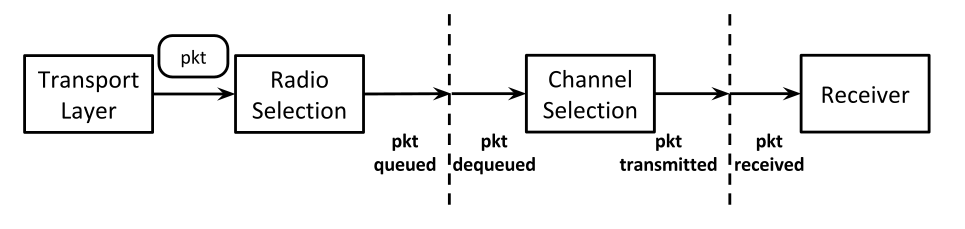
\includegraphics[width=1.0\textwidth]{myFigures/blockDiagram.png}
        \caption{Operational block diagram of our proposed feedback-based multi-radio exploitation approach}
        \label{fig:blockDiagram}
    \end{center}
\end{figure}

Figure~\ref{fig:blockDiagram} depicts the operational steps of our proposed feedback-based multi-radio exploitation approach. When a transport layer packet is received on the data link layer, our proposed approach first selects the radio to take the responsibility of transmitting the packet. This radio selection process is performed based on two radio counters, the number of total packets queued on the radio and the number of total packets transmitted by the radio. After selecting the radio, our secondary user agent enqueues the packet on the corresponding selected radio queue. It is to be noted here that, the channel selection process is not performed at that time. The channel is selected only after the dequeuing of the packet. After the packet is dequeued from the selected radio's queue, the radio senses its currently assigned channel for primary user activity. If the radio senses that there is no primary user on that channel the packet is transmitted on that channel. However, if the primary user is active on that channel, the radio has to switch to another channel. Only then, the channel selection process is performed to find another channel to which the radio senses next for primary user activity. This channel selection process is conducted based on two channel counters, the number of total packets transmitted by the corresponding secondary user on the channel and the number of total packets successfully received by the receiver on the channel.

We implement our proposed feedback-based approach in \texttt{ns-3} to evaluate its performance in terms of throughput along with delay and drop ratio. Our simulation results demonstrate that the proposed approach can achieve significant improvement in network throughput in addition to improving other performance metrics in most of the cases.

% Summary of Contributions
%Then have a final paragraph or subsection: "Summary of Contributions". It should list the major contributions in bullet form, mentioning in which sections they can be found. This material doubles as an outline of the rest of the paper, saving space and eliminating redundancy.

\section{Summary of Contributions}

Based on our study in this thesis, we make the following set of contributions:

\begin{itemize}
\item We propose a feedback-based multi-radio exploitation approach, along with several variants, to solve the throughput degradation problem in MRCRNs. In our proposed approach, performance information obtained from lower layers (Physical layer and Data link layer) is incorporated in the process of upper layer (Application layer) decision making on radio and channel selection.
\item We evaluate the performance of our proposed approach through discrete-event simulation. We implement the proposed approach and its variants in \texttt{ns-3} to demonstate efficacy of their radio selection and channel selection policies, and measure various performance metrics in response to an increase in the number of radios per SU.
\item We compare performance of our proposed approach against that of existing approaches in the literature. Comparative results confirm significant improvement over existing approaches through using our proposed approach. Our proposed approach increases total network throughput by 51\%, decreases packet drop ratio by 35\%, and decreases end-to-end delay by 13\% on an average against that of other existing approaches.
%\item At last, we also provide several research questions in the domain of MRCRNs to guide future research direction.
\end{itemize}
\endinput
